\documentclass[a4paper]{article}

%% Language and font encodings
\usepackage[english]{babel}
\usepackage[utf8x]{inputenc}
\usepackage[T1]{fontenc}

%% Sets page size and margins
\usepackage[a4paper,top=3cm,bottom=2cm,left=3cm,right=3cm,marginparwidth=1.75cm]{geometry}

%% Useful packages
\usepackage{amsmath}
\usepackage{graphicx}
\usepackage[colorinlistoftodos]{todonotes}
\usepackage[colorlinks=true, allcolors=blue]{hyperref}

\title{Reporte de Actividad 7}
\author{Valenzuela Terán Jonás}

\begin{document}
\maketitle

\section{Introducción}

En esta actividad se continua con el tema anterior, agregando no linealidad, amortiguamiento y forzamiento, los cuales crean patrones más complicados e interesantes. Además, adaptando el modelo a estos parámetros, da una mejor comprensión de como el modelo funciona en el código.


\section{Resumen de artículo: Coupled spring equations}

\subsection{Introducción}

La perspectiva general con la que se toma a las ecuaciones diferenciales esta cambiando mucho, de realizar técnicas para encontrar soluciones analíticas a visualizar y resolver numéricamente estas con las herramientas disponibles.

En el articulo, se trabaja con el problema de 2 resortes y 2 masas conectadas en serie, suponiendo que obedecen la Ley de Hooke. Esto introduce 2 ecuaciones diferencial linear de segundo orden. Hacer esto permite tener una interpretación física clara de la fase, amplitud, periodicidad, y la sensibilidad del sistema a las condiciones iniciales al introducir no linealidad.

\subsection{El modelo del doble resorte}

El modelo consiste en 2 resortes $k_1$ y $k_2$, y 2 masas $m_1$ y $m_2$ conectados en serie.

\subsubsection{Asumiendo la Ley de Hooke}

Suponiendo que  cumple la Ley de Hooke en el sistema, las fuerzas restauradoras producto de las elongaciones son de la forma $-k_1 l_1$ y $-k_2 l_2$ ($l$ siendo la elongación de cada resorte), la masa inferior solo siente la fuerza del resorte 2 $-k_2 (x_2 - x_1)$, donde $x_2 - x_1 = l_2$, mientras que la masa superior siente esta y la del resorte superior $-k_1 x_1$, donde $x_1 = l_1$. Escribimos las ecuaciones para las fuerzas de la forma:

\begin{center}
	$m_1 \ddot{x}_1 = - k_1 x_1 - k_2 (x_2 - x_1)$

	$m_2 \ddot{x}_2 = -k_2 (x_2 - x_1)$
\end{center}

Se tiene un par de ecuaciones diferenciales lineales de segundo orden, para obtener una ecuación de $x_1$ sin involucrar a $x_2$, se despeja de la ecuación:

\begin{center}
	$x_2 = -\frac{m_1 \ddot{x_1}}{k_2} + \frac{k_1 + k_2}{k_2} x_1$
\end{center}

una ecuación de segundo orden, la sustituimos en la segunda ecuación:

\begin{center}
$m_1 m_2 {x_1}^{(4)} + (m_2 k_1 + k_2 (m_1 + m_2)) \ddot{x}_1 + k_1 + k_2 x_1 = 0$
\end{center}

análogamente para $x_2$

\begin{center}
$m_1 m_2 {x_2}^{(4)} + (m_2 k_1 + k_2 (m_1 + m_2)) \ddot{x}_2 + k_1 + k_2 x_2 = 0$
\end{center}

Las 2 masas obedecen la misma ecuación, que solo necesita las 2 velocidades y posiciones iniciales para resolverla.  Podemos usar esta ecuación en la forma de 2 ecuaciones diferenciales de primer grado, con $v_1 = \ddot{x}_1$, $v_2 = \ddot{x}_2$.

\begin{center}
$v_1 = -\frac{k_1}{m_1} - \frac{k_2}{m_1} (x_1 - x_2)$

$v_2 = -\frac{k_2}{m_2} (x_2 - x_1)$
\end{center}

\subsubsection{Algunos ejemplos con masas iguales}

Se considera un modelo con $m_1 = m_2 = 1$, en el caso de no tener amortiguamiento, la ecuación característica es:

\begin{center}
$m^4 + (k_1 + 2 k_2) m_2 + k_1 k_2 = 0$
\end{center}

que tiene raíces: 

\begin{center}
$\pm \sqrt[]{-\frac{1}{2} k_1 - k_2 \pm \frac{1}{2} \sqrt[]{{k^2}_1 +4 {k^2}_2}}$
\end{center}


El ejemplo 2.1 plantea el sistema con $k_1 = 6$, $k_2 = 4$, y $(x_1(0),v_1(0),x_2(0),v_2(0)) = (1,0,2,0)$. Se obtiene, mediante lo desarrollado, la solución analítica:

\begin{center}
$x_1(t) = \cos \sqrt[]{2} t$

$x_2(t) = 2 \cos \sqrt[]{2} t$
\end{center}

Se observa que el movimiento para ambas masas es en fase, solo sus amplitudes son diferentes, las gráficas del movimiento y fase muestran patrones simples, estas se encontrarán en la sección \textit{Implementación en python (jupyter lab)}.

El ejemplo 2.2 tiene condiciones iniciales $k_1 = 6$, $k_2 = 4$, y $(x_1(0),v_1(0),x_2(0),v_2(0)) = (-2,0,1,0)$, que resulta en un movimiento completamente fuera de fase, las soluciones analíticas obtenidas, útiles en nuestro contexto para verificar el error de soluciones numéricas, son:

\begin{center}
$x_1(t) = -2 \cos 2 \sqrt[]{3} t$

$x_2(t) = \cos 2 \sqrt[]{3} t$
\end{center}

El ejemplo 2.3 tiene condiciones iniciales $k_1 = 0.4$, $k_2 = 1.808$, y $(x_1(0),v_1(0),x_2(0),v_2(0)) = (0.5,0,-0.5,0.7)$, aqui ocurre un movimiento más elaborado que los 2 anteriores, debido a que no entran completamente en fase o no fase, además, los valores de $k$ fueron seleccionados cuidadosamente para que ocurriera.

\subsubsection{Amortiguamiento}

Agregamos el amortiguamiento en las ecuaciones, introduciendo una fuerza que depende solamente de la velocidad de la masa, y coeficientes de fricción ${\delta}_1$ y ${\delta}_2$.

\begin{center}
	$m_1 \ddot{x}_1 = -{\delta}_1 v_1 - k_1 x_1 - k_2 (x_2 - x_1)$

	$m_2 \ddot{x}_2 = -{\delta}_2 v_2 -k_2 (x_2 - x_1)$
\end{center}

El ejemplo 2.4 introduce amortiguamiento, con condiciones iniciales $k_1 = 0.4$, $k_2 = 1.808$, ${\delta}_1 = 0.1$, ${\delta}_1 = 0.2$ y $(x_1(0),v_1(0),x_2(0),v_2(0)) = (1,0.5,2,0.5)$. Se observa como el movimiento es periódico pero pierde amplitud, sin embargo, la fase varía considerablemente.

\subsection{Agregando no linearidad}

Si suponemos que la fuerza producida por el resorte es no lineal, que la mayor parte del tiempo es asi para vibraciones grandes, agregamos un término no lineal a la fuerza, de tal manera que la fuerza tiene la forma:

\begin{center}
$-kx + \mu x^3$
\end{center}

El modelo se convierte en:

\begin{center}
	$m_1 \ddot{x}_1 = -{\delta}_1 v_1 - k_1 x_1 - k_2 (x_2 - x_1) + {\mu}_1 {x^3}_1 + {\mu}_2 (x_1 - x_2)^3$

	$m_2 \ddot{x}_2 = -{\delta}_2 v_2 -k_2 (x_2 - x_1) + {\mu}_2 (x_2 - x_1)^3$
\end{center}

El rango de posibilidad de movimientos del modelo no lineal es mucho mas grande y complicado que el lineal, además, soluciones numéricas no pueden asegurar presición para intervalos de tiempo grandes, debido a redondeo, truncamiento, propagación de error, etc.

El ejemplo 3.1 tiene condiciones iniciales $m_1 = m_2 = 1$, $k_1 = 0.4$, $k_2 = 1.808$, ${\delta}_1 = 0$, ${\delta}_2 = 0$, ${\mu}_1 = -\frac{1}{6}$, ${\mu}_2 = -\frac{1}{10}$ y $(x_1(0),v_1(0),x_2(0),v_2(0)) = (1,0,0.5,0)$, Muestra un movimiento donde se presenta la no linealidad, pero debido a que no existe amortiguamiento, el movimiento es oscilante y parece ser periódico sin cambios bruscos.

El ejemplo 3.2 tiene condiciones $k_1 = 0.4$, $k_2 = 1.808$, ${\delta}_1 = 0$, ${\delta}_2 = 0$, ${\mu}_1 = -\frac{1}{6}$, ${\mu}_2 = -\frac{1}{10}$ y $(x_1(0),v_1(0),x_2(0),v_2(0)) = (-0.5,0.5,3.001,5.9)$. Se observa un movimiento muy diferente a lo que se ha visto anteriormente, produciendo patrones interesantes.

El ejemplo 3.3 es similar al anterior, pero se cambia la posición inicial de $m_1$ por $x_1(0) = -0.6$, una diferencia de 0.1, sirve para mostrar la sensibilidad del modelo a condiciones iniciales, y como produce resultados muy diferentes. 

\subsection{Agregando forzamiento}

Es relativamente fácil agregar una fuerza externa al modelo, es posbile hacerlo con fuerzas diferentes para cada masa, si agregamos una fuerza sinusoidal, tenemos que:

\begin{center}
	$m_1 \ddot{x}_1 = -{\delta}_1 v_1 - k_1 x_1 - k_2 (x_2 - x_1) + {\mu}_1 {x^3}_1 + {\mu}_2 (x_1 - x_2)^3 + F_1 \cos {\omega}_1 t$

	$m_2 \ddot{x}_2 = -{\delta}_2 v_2 -k_2 (x_2 - x_1) + {\mu}_2 (x_2 - x_1)^3 + F_2 \cos {\omega}_2 t$
\end{center}

El rango de movimientos posible por este modelo es aún más grande, podemos esperar resonancia, soluciones armónicas, subarmónicas y aquellas que tienen un limite para la gráfica de fase.

El ejemplo 4.1 toma $m_1 = m_2 = 1$,  $k_1 = \frac{2}{5}$, $k_2 = 1$, ${\delta}_1 = \frac{1}{10}$, ${\delta}_2 = \frac{1}{5}$, ${\mu}_1 = \frac{1}{6}$, ${\mu}_2 = \frac{1}{10}$, $F_1 = \frac{1}{3}$, $F_2 = \frac{1}{5}$, ${\omega}_1 = 1$, ${\omega}_2 = \frac{3}{5}$ y $(x_1(0),v_1(0),x_2(0),v_2(0)) = (-0.7,0,0.1,0)$. Debido al amortiguamiento, se esperan movimientos diferentes para valores pequenos y grandes de t, ya que para valores grande de t se podrá ver un límite en el ciclo para la fase (desplazamiento contra velocidad).


\section{Implementación en python (jupyter lab)}

Al igual que la práctica anterior, se realizó la gráfica para desplazamiento contra tiempo, desplazamiento 1 contra desplazamiento 2, y fase (desplazamiento contra velocidad) para los ejemplos 3.1, 3.2, 3.3 y 4.1, en estos casos no fue posible calcular el error relativo ya que no se cuenta con una solución analítica. A continuación se muestran las gráficas obtenidas usando el entorno de programación jupyter lab con lenguaje python y librerias para graficación y solución numérica:

\vspace{0.5cm}

\textit{Ejemplo 3.1}

\begin{center}
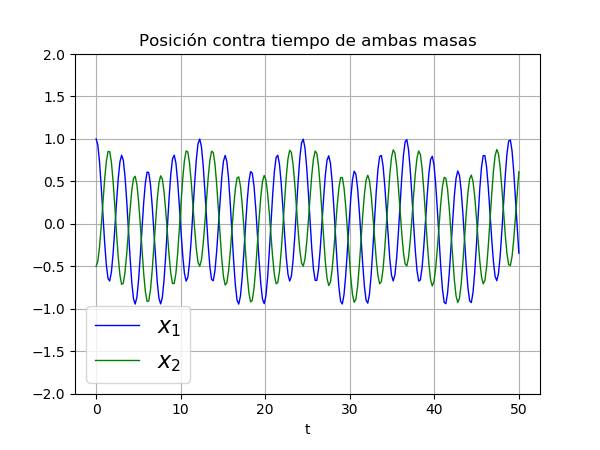
\includegraphics[height=6cm]{ejemplo3-1.png}

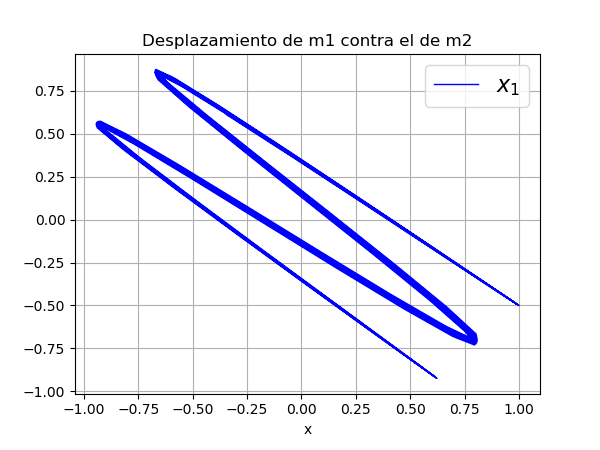
\includegraphics[height=6cm]{recta3-1.png}

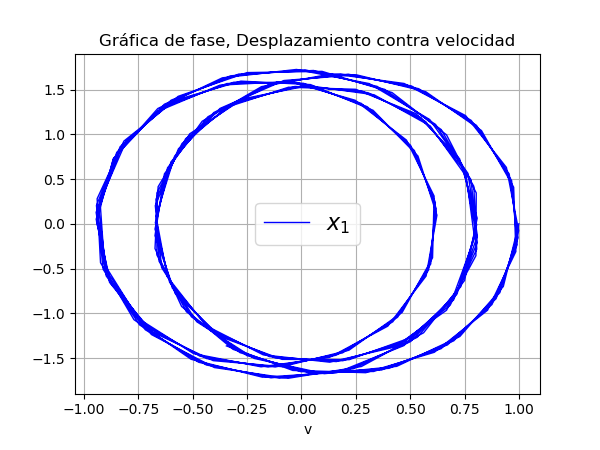
\includegraphics[height=6cm]{circulo3-1-1.png}

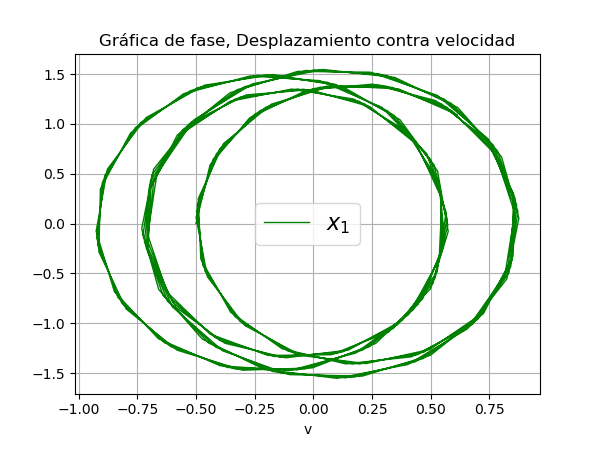
\includegraphics[height=6cm]{circulo3-1-2.png}
\end{center}

\textit{Ejemplo 3.2}

\begin{center}
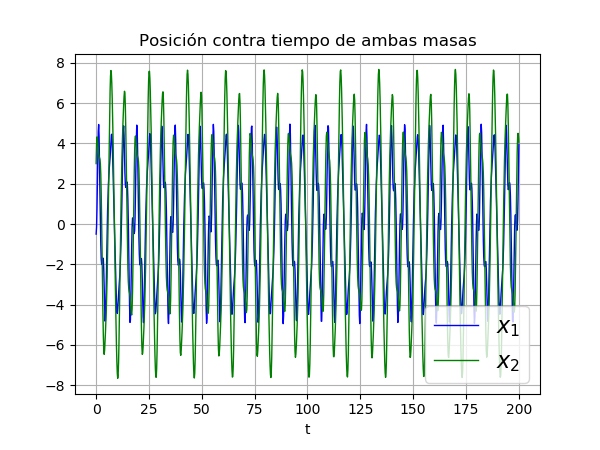
\includegraphics[height=6cm]{ejemplo3-2.png}

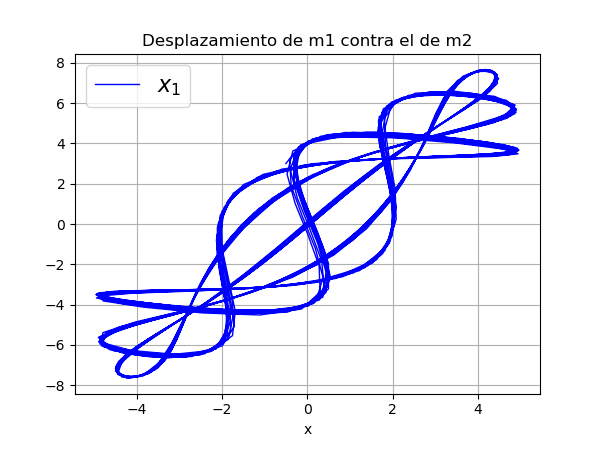
\includegraphics[height=6cm]{recta3-2.png}

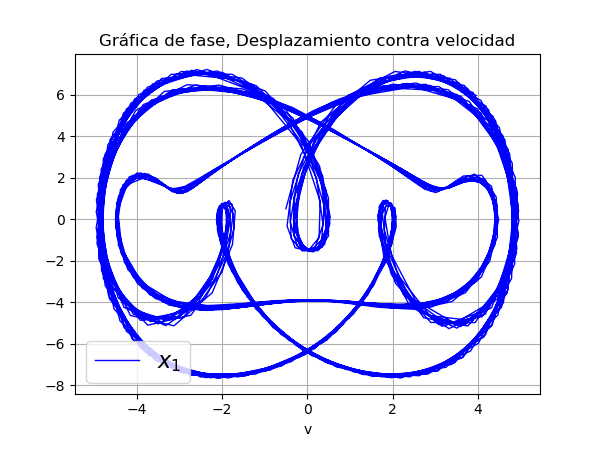
\includegraphics[height=6cm]{circulo3-2-1.png}

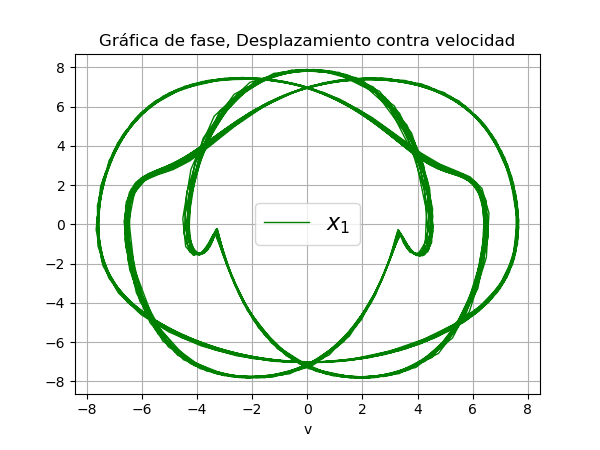
\includegraphics[height=6cm]{circulo3-2-2.png}
\end{center}

\textit{Ejemplo 3.3}

\begin{center}
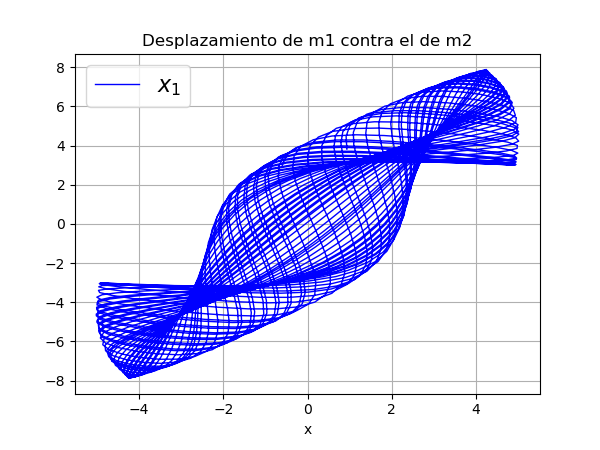
\includegraphics[height=6cm]{recta3-3.png}

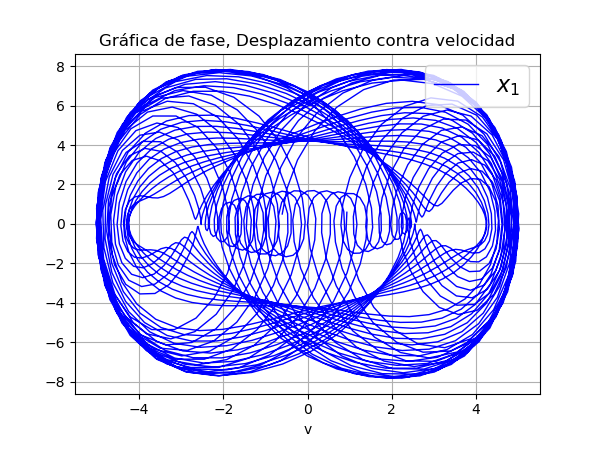
\includegraphics[height=6cm]{circulo3-3-1.png}

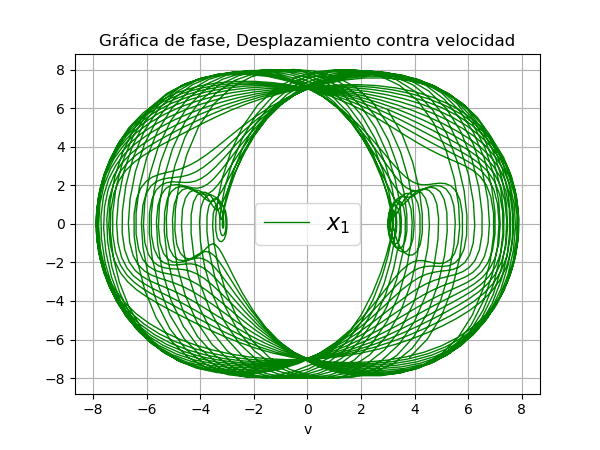
\includegraphics[height=6cm]{circulo3-3-2.png}
\end{center}

\textit{Ejemplo 4.1}

\begin{center}
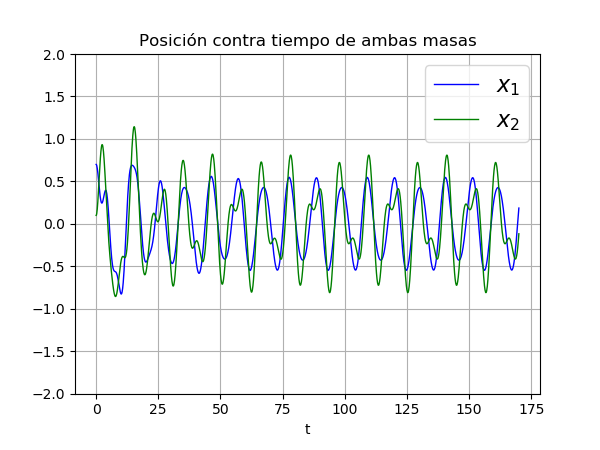
\includegraphics[height=6cm]{ejemplo4-1.png}

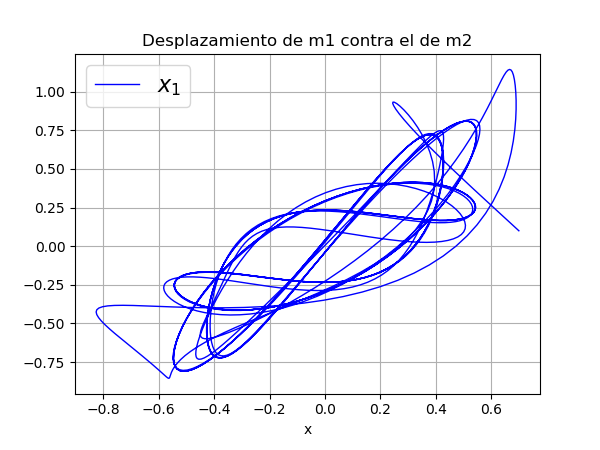
\includegraphics[height=6cm]{recta4-1.png}

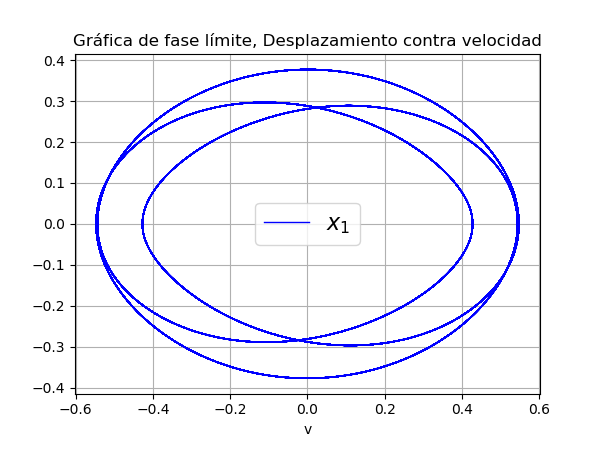
\includegraphics[height=6cm]{circulo4-1-1l.png}

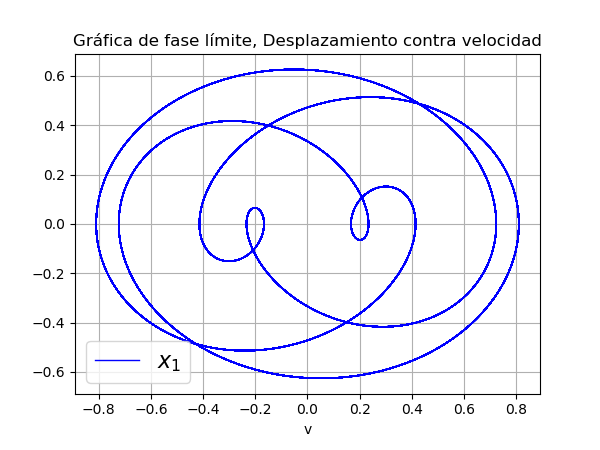
\includegraphics[height=6cm]{circulo4-1-2l.png}
\end{center}

En el ejemplo 4.1 se muestra las imagenes límite que tiene la fase, al graficar datos sólo con valores de t grande.

Para realizar cada ejemplo se siguió un proceso similar, adaptando el modelo para que aceptara no linearidad y forzamiento al definirlo:

\begin{itemize}
\item Definir el modelo, declarando parámetros y especificando la función involucrada
\item Brindar valor a los parámetros, condiciones iniciales, y especificar el tiempo, tolerancia y número de puntos que se generan, escribiendo estos en un archivo.
\item Recuperar los resultados del archivo y especificar los ejes de lo que se desea graficar.
\end{itemize}

\section{Conclusiones}

Se mostró como agregando más consideraciones, un modelo cíclico se vuelve no lineal, creando patrones más interesantes y que estos tienden a un movimiento, y que las herramientas utilizadas ayudan mucho con el manejo de una gran cantidad de datos de este tipo.


\section{Bibliografía}

\begin{itemize}
\item 	SARAH DUNCAN GRAHAM. (2003). Coupled spring equations. 8 de Marzo, 2018, de University of Southern Mississippi Sitio web: 
\textit{http://math.oregonstate.edu/\~gibsonn/Teaching/MTH323-010S15/Supplements/coupled\_spring.pdf}

\item (2009). Coupled spring-mass system. 8 de marzo, 2018, de SciPy Cookbook Sitio web: 
\textit{http://scipy-cookbook.readthedocs.io/items/CoupledSpringMassSystem.html}
\end{itemize}


\section{Apéndice}

\begin{itemize}
\item     ¿Qué más te llama la atención de la actividad completa? ¿Qué se te hizo menos interesante?

El comportamiento del sistema de doble resorte, que puede complicarse mucho.

\item     ¿De un sistema de masas acopladas como se trabaja en esta actividad, hubieras pensado que abre toda una nueva área de fenómenos no lineales?

No, el oscilador armónico del resorte singular hace parecer que el fenómeno es muy sencillo y que no hay mucho por estudiar.

\item     ¿Qué propondrías para mejorar esta actividad? ¿Te ha parecido interesante este reto?

Sería interesante ver como cambia el sistema al modificar ligeramente un parámetro, con una especie de deslizador, parecido como el que es visto en GeoGebra.

\item     ¿Quisieras estudiar mas este tipo de fenómenos no lineales?

Si, y ver los patrones interesantes que produce.

\end{itemize}



\end{document}